% 2015_national_paper_1_liberal_q18_fig1: 菱形ABCD, G为对角线交点, BE垂直平面, E在B正上方
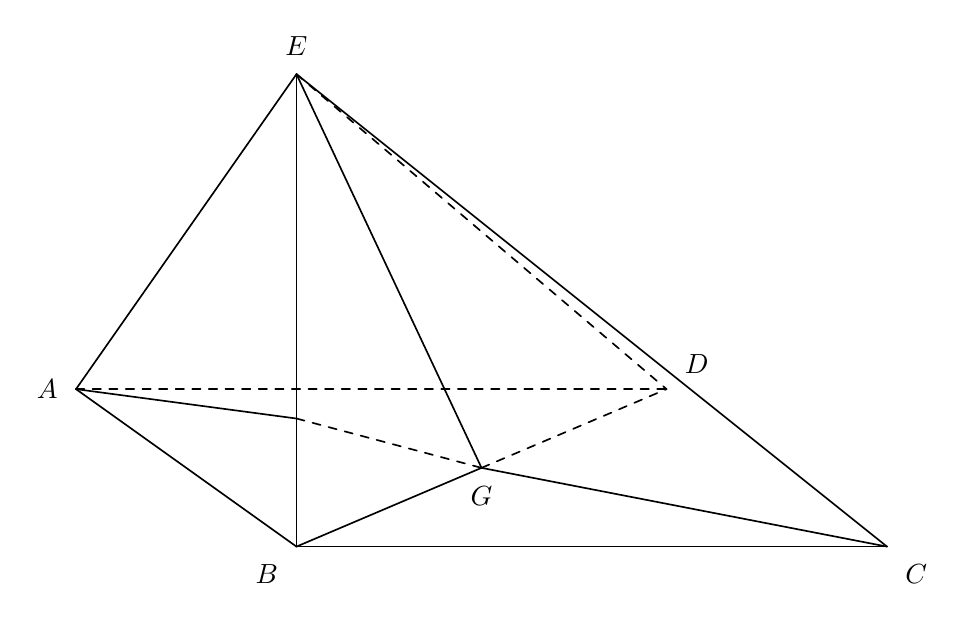
\begin{tikzpicture}[line width=0.6pt, line join=round, line cap=round, font=\normalsize]
\coordinate (E) at (2.0000000000,6.0000000000);
\coordinate (A) at (-0.8000000000,2.0000000000);
\coordinate (B) at (2.0000000000,0.0000000000);
\coordinate (C) at (9.5000000000,0.0000000000);
\coordinate (D) at (6.7000000000,2.0000000000);
\coordinate (G) at (4.3500000000,1.0000000000);
% 侧棱
\draw (E) -- (A);
\draw (E) -- (B);
\draw (E) -- (G);
\draw (E)--(C);\draw[dashed] (E)--(D);
% E-C顶部被遮挡段(虚线,与实线共线,取E向C约30%处)

% 底面菱形
\draw (A) -- (B);
\draw (B) -- (C);
\draw (B) -- (G);
\draw (A)--(2,1.6266666667);\draw[dashed] (2,1.6266666667)--(G);
\draw (G) -- (C);
\draw[dashed] (G) -- (D);
\draw[dashed] (A) -- (D);
% 标签(避碰外置)
\node[above, yshift=3.0pt] at (E) {$E$};
\node[left, xshift=-3pt] at (A) {$A$};
\node[below left, xshift=-3.0pt, yshift=-3.0pt] at (B) {$B$};
\node[below right, xshift=3.0pt, yshift=-3.0pt] at (C) {$C$};
\node[above right, xshift=3.0pt, yshift=2.0pt] at (D) {$D$};
\node[below, yshift=-3pt] at (G) {$G$};
\end{tikzpicture}
